\documentclass{article}
\usepackage{preamble}
\input{preamble}
\graphicspath{ {images/} }
%%%%%%%%%%%%%%%% Document %%%%%%%%%%%%%%%%
\begin{document}
\begin{center}
{\huge \underline{Variational Auto Encoders}}
\end{center}
\section{Introduction}
\begin{definition}[Statistical Inference] Determining properties of the underlying probability distribution based on observed data. This could include estimating parameters, latent variables, or making predictions. In Bayesian inference, the primary goal is to compute the posterior $p(z|x)$:

\[
  p(z|x) = \frac{p(x,z)}{p(x)} = \frac{p(x|z) p(z)}{\int_{\mathcal{Z}} p(x,z) \d{z} }
\]
Since the marginal likelihood $p(x)$ is intractable, we instead approximate the posterior $p(z|x)$ with a simpler, tractable distribution $q(z| \lambda)$, and we wish to minimize the KL divergence $KL \Big( q(z | \lambda) \, || \, p(z | x) \Big)$, or equivalently maximize the Evidence Lower Bound (ELBO):


\end{definition}
\begin{definition}[Density Estimation] Approximating PDF $p(x)$ of a random variable $X$ based on observed data $\left\{ x_1, \ldots, x_n \right\}$ drawn i.i.d from the underlying distribution. Can be either parametric, e.g.
\[
  p(x | \theta) \sim  \mathcal{N}( \mu_x, \sigma_x)
\]
or nonparametric density estimation, for example Kernel Density Estimation:
\[
  p(x) = \frac{1}{n h^{d}} \sum_{i=1}^{n} K \left( \frac{x-x_i}{h} \right) 
\]
\end{definition}
\begin{definition}[Modeling] Modeling is unveiling the underlying ruling processes, by posing hypotheses and predictions, based on observations. For instance, physicists model how fluids flow, and biologists the  structure of organisms. 

Modeling often involves representation, where we describe a phenomena using specific qualities and quantities related to the process we are interested in. We describe an object by its shape, color, position, volume, etc. 
When looking at data - a large collection of samples - in some cases, it is reasonable to believe that those representations follow some distributions. For example, human height clearly follow some probability distribution. In such cases, we can think of the samples as being "generated" from those distributions. When such a hypothesis is true, we can generate new samples in the population, provided we estimated its probabilities. Alternatively, we may say that we have uncertainty about those variables, and we specify the degree and nature of this uncertainty  in terms of probability distributions.  
\end{definition}

\begin{remark} A complete probabilistic model captures both the \ul{distributions} of its components and the \ul{relations/dependencies} between them. Usually the linear relations, given by the covariances.
\end{remark}

\begin{definition}[Probabilistic Model] Assume the observed variables $\bm{x}$ are a random sample from an unknown underlying process, whose true probability distribution is $p^{\ast}(\bm{x})$. We approximate this underlying process with a chosen probabilistic model $p_{\theta}(\bm{x})$, with parameters $\bm{\theta}$:
\[
  \bm{x} \sim p_{\theta}(\bm{x}) 
\]
  Learning is the process of searching for a value of the parameters $\theta$, such that the probability function given by the mode $p_{\theta}(\bm{x})$, approximates the true distribution of the data, denoted by $p^{^{\ast}}(\bm{x})$, such that for any observed $\bm{x}$:
\[
  p_{\theta}(\bm{x}) \approx p ^{\star}(\bm{x}) 
\]
\end{definition}

\begin{definition}[Conditional Models] Often, we are not interested in learning an unconditional model $p_{\theta}(\bm{x})$, but a conditional model $p_{\theta}(\bm{y} | \bm{x})$, that approximates the underlying conditional distribution $p ^{\ast}(\bm{y} | \bm{x})$: A distribution over the values of variable $\bm{y}$, conditioned on the value of an observed variable $\bm{x}$. $\bm{x}$ is often called the \textit{input} of the model. 

A common example is image classification, where $\bm{x}$ is the image, and $\bm{y}$ is the label, and $p_{\theta}(\bm{y}|\bm{x})$ is chosen to be the categorical distribution, whose parameters are computed from $\bm{x}$. 
\end{definition}

\begin{remark} We can use neural networks to parameterize a distribution. For example for the categorical distribution $\mathrm{Categorical}(y ; \bm{p})$ over a class label $y$, we have: 
\begin{gather*}
  \bm{p} = \mathrm{NeuralNet}(\bm{x}) \\
  p_{\theta}(y | \bm{x}) = \mathrm{Categorical}(y ; \bm{p})
\end{gather*}
\end{remark}

\subsection{Directed PGMs and NNs}
We work with \textit{directed} PGMs, where all variables are organized into a directed acyclic graph, and the joint distribution over the variables factorizes as a product of prior and conditional probabilities:
\[
  p_{\theta}(\bm{x}_1, \ldots  \bm{x}_m) = \sum_{j=1}^{m} p_{\theta}(\bm{x}_j | Pa(\bm{x}_j))    
\]
where $Pa(\bm{x}_j)$ is the set of parent variables of node $j$ in the directed graph. 

Traditionally, each conditional probability distribution $p_{\theta}(\bm{x}_j | Pa(\bm{x}_j))$ is parameterized by a lookup table or a linear model. A more flexible way is to parametrize such conditional distributions using a neural network. In this case, the NN takes as input the parents of a variable, and produce the distributional parameters $\bm{\eta}$ over that variable:
\begin{gather*}
  \bm{\eta} = \mathrm{NeuralNet}(Pa(\bm{x})) \\
  p_{\theta}(\bm{x} | Pa(\bm{x})) = p_{\theta}(\bm{x} | \bm{\eta}) 
\end{gather*}
for example, in VAE, when learning $p_{\theta}(\bm{x} | \bm{z})$, note that  $Pa(\bm{x}) = \bm{z}$, and the recognition model learn the distributional parameters $\bm{\eta}  = (\mu, \sigma)$  to parametrize $p_{\theta}(\bm{x} | \bm{\eta})$
\subsection{Learning in Fully Observed Models with Neural Nets}

If all variables in the directed model are observed in the data, then we can compute and differentiate the log-probability of the data under the model, leading to a relatively straightforward optimization. 

\ul{Dataset}: We collect a dataset $\mathcal{D}$ consisting of $N$ datapoints:
\[
  \mathcal{D} = \left\{ \bm{x}^{(1)}, \ldots, \bm{x}^{(N)} \right\} 
\]
The datapoints are assumed to be independent samples from an unchanging underlying distribution, i.e. i.i.d. Then the probability of the datapoints given the parameters factorizes as a product of individual datapoint probabilities:
\[ \begin{array}{@{} R{0.3\textwidth}  C{0.6\textwidth} P{0.1\textwidth} @{}} 
& \[
 \log p_{\theta}(\mathcal{D})  = \displaystyle \sum_{\bm{x} \in \mathcal{D}} \log  p_{\theta}(\bm{x}) \label{eq:log_likelihood} \tag{Maximum Likelihood}
\]  &   
\end{array} \]

A common criterion for probabilistic models is maximum log-likelihood (MLL). We attempt to find the parameters $\theta$ that maximize the above sum, or equivalently, the average, of the log-probabilities assigned to the data by the model. Since our model is limited by its expressiveness, and our data is noisy, this can not be trivially solved.  

Using stochastic gradient descent, we draw a minibatch $\mathcal{M}$ of the data, and since:
\[
  \nabla_{\theta} \log  p_{\theta}(\mathcal{D})  \simeq \nabla_{\theta} \log  p_{\theta} (\mathcal{M})  = \sum_{\bm{x} \in \mathcal{M}} \nabla_{\theta}  \log  p_{\theta}(\bm{x})
\]
where $\simeq$ indicates an unbiased estimator, we can use $\displaystyle \sum_{\bm{x} \in \mathcal{M}} \nabla_{\theta} \log  p_{\theta}(\bm{x})$ to iteratively update $\theta$ and  hill-climb to a local optimum of the~\ref{eq:log_likelihood}.  

\subsection{Learning and Inference in Deep Latent Variable Models}
\begin{definition}[Latent Variables]  Variables which are part of the model, but which we do not observe.

For an observed variable $\bm{x}$ and an unobserved variable $\bm{z}$, the joint distribution is denoted $p_{\theta}(\bm{x}, \bm{z})$ over both variables. The marginal distribution over the observed variables $p_{\theta}(\bm{x})$ is given by:
  \begin{equation} \label{eq:marginalLikelihood}
  p_{\theta}(\bm{x}) = \int p_{\theta}(\bm{x}, \bm{z}) \d{\bm{z}}
\end{equation}
This is also called the \textit{evidence}.
\end{definition}

\begin{definition}[Deep Latent Variable Model (DLVM)]  latent variable model $p_{\theta}(\bm{x}, \bm{z})$ whose distributions are parameterized by neural nets. Then, even when each factor (prior or conditional distribution) in the directed model is relatively simple (such as a conditional Gaussian), the marginal distribution $p_{\theta}(\bm{x})$ can be very complex. This expressivity makes DLVM attractive for approximating complicated underlying distributions $p ^{\star}(\bm{x})$. 
\end{definition}

\begin{example}  A simple DLVM is:
\[
  p_{\theta}(\bm{x}, \bm{z}) = p_{\theta}(\bm{z}) p_{\theta}(\bm{x} | \bm{z}) 
\]
we call $p_{\theta}(\bm{z})$ the \textit{prior distribution} over $\bm{z}$. 

  For example, assume, for binary data $\bm{x}$ (such as 0-1 MNIST images), a spherical Gaussian latent space, and a factorized Bernoulli observation model. Then:
\begin{gather*}
  p (\bm{z}) = \mathcal{N}( \bm{z} ; 0, I) \\
  \bm{p} = \mathrm{DecoderNeuralNet}_{\theta} (\bm{z}) \\
  \log p( \bm{x} | \bm{z}) = \sum_{j=1}^{D} \log  p (x_j | \bm{z}) = \sum_{j=1}^{D} \log \mathrm{Bernoulli}( x_{j} ; p_{j} )
\end{gather*}
where $D$ is the dimensionality of $\bm{x}$. 
\end{example}

\begin{remark} As $\bm{z}$ is not observed, computing~\cref{eq:marginalLikelihood} is intractable, and hence we cannot directly optimize it. 

  For a Fully observed model, like $p_{\theta}(\bm{x}) \sim \mathcal{N}( \mu, \sigma ^2)$, we can easily compute $\log p_{\theta}(\bm{x})$, and optimize $\theta$ using the gradients of~\ref{eq:log_likelihood}. 

For latent variable models, we have:
\[
  p_{\theta}(\bm{x}) = \int p_{\theta}(\bm{x}, \bm{z}) \d{\bm{z}}
\]
The integral over $\bm{z}$ often lacks a closed-form solution, due to the complexity of taking its gradient,  and the dimensionality of $\bm{z}$. 

  Note - we often do know $p_{\theta}(\bm{x}, \bm{z})$, the joint distribution, since we have $p_{\theta}(\bm{x}, \bm{z}) =  p_{\theta}(\bm{x} | z) p_{\theta}(\bm{z})$, and we often assume $p_{\theta}(\bm{z})$, and $p_{\theta}(\bm{x} | z)$, the \textit{likelihood} 

The intractability of $p_{\theta}(\bm{x})$ is related to the intractability of the \textit{posterior} distribution $p_{\theta}(\bm{z} | \bm{x})$, via the identity:
\[
  p_{\theta}(\bm{z} | \bm{x}) = \frac{p_{\theta}(\bm{x}, \bm{z})}{ p_{\theta}(\bm{x})}
\]
  since $p_{\theta}(\bm{x}, \bm{z})$ is tractable to compute. We approximate $p_{\theta}(\bm{z} | \bm{x})$ using variational inference, by a similar distribution $q \theta(\bm{z} | \bm{x})$, called the \textbf{variational distribution}. 
\end{remark}

\section{Variational Auto Encoders}
\begin{remark}[Motivation] Suppose we have observed data \(\mathbf{x}\), for instance, pixels of dog images. These data points are drawn from some true but unknown distribution \(p^{\ast}(\mathbf{x})\). Our goal is to approximate $p ^{\ast}(\bm{x})$ using a parameterized family \(p_{\theta}(\mathbf{x})\), enabling tasks like generation (sampling new images) or downstream inference (classification, etc.).

Directly modeling \(p_{\theta}(\mathbf{x})\) can be extremely challenging, especially for complex, high-dimensional data. One common approach is to introduce latent variables \(\mathbf{z}\) that describe underlying factors or structures, and then express the data distribution through marginalization:
\[
p_{\theta}(\mathbf{x}) = \int p_{\theta}(\mathbf{x} \mid \mathbf{z}) p_{\theta}(\mathbf{z})\,d\mathbf{z}.
\]

Here, \(p_{\theta}(\mathbf{x}\mid\mathbf{z})\) is often simpler to model than \(p_{\theta}(\mathbf{x})\) itself. For example, \(\mathbf{z}\) might represent attributes like a dog's breed, pose, or lighting, making it easier to build a model that generates images \(\mathbf{x}\) given \(\mathbf{z}\). We also choose a prior \(p_{\theta}(\mathbf{z})\) that is tractable, such as a Gaussian.

The challenge is that computing \(p_{\theta}(\mathbf{x})\) requires integrating over \(\mathbf{z}\), which is typically intractable for complex models. This makes it hard to directly optimize parameters \(\theta\) by maximum likelihood.

\textbf{Role of the Posterior and Variational Inference}:
  Remember our goal is to find parameters $\theta$ that will optimize $\log p_{\theta}(\bm{x})$. Using mathematical tricks, we use posterior $p_{\theta}(\bm{z} | \bm{x})$ - in fact an approximation $q_{\phi}(\bm{z} | \bm{x})$ - and by choosing $\phi$ such that $q_{\phi}( \bm{z} | \bm{x})$ is close to $p_{\theta}(\bm{z})$, we increase $\log p_{\theta}(\bm{x})$. 

Specifically, note that:
\[
  \log p_{\theta}(\bm{x}) = \log \int p_{\theta}(\bm{x} | \bm{z}) p_{\theta}(\bm{z}) \d{\bm{z}}
\]

We multiply and divide by  $q_{\phi}(\bm{z} | \bm{x})$:
\[
  \log p_{\theta}(\bm{x}) = \log \int q_{\phi}(\bm{z} | \bm{x}) \frac{ p_{\theta}(\bm{x}, \bm{z})}{q_{\phi}(\bm{z} | \bm{x})} \d{\bm{z}}
\]
Recall Jensen's inequality for concave function states that $f(E[X]) \geq E[f(X)]$, and since $\log$ is concave, we get that $\log E[X] \geq E [\log X]$. Define $X = \frac{p_{\theta}(\bm{x}, \bm{z})}{q_{\phi}(\bm{z} | \bm{x})}$, and we get:
\[
  \log p_{\theta}(\bm{x}) \geq \int q_{\phi}(\bm{z} | \bm{x}) \log \frac{p_{\theta}(\bm{x}, \bm{z})}{q_{\phi}(\bm{z} | \bm{x})} \d{\bm{z}}
\]

Rewrite the integrand using $p_{\theta}(\bm{x}, \bm{z}) = p_{\theta}(\bm{x} | \bm{z}) p_{\theta}(\bm{z})$ and we get:
\[
\log p_{\theta}(\bm{x}) \geq \int q_{\phi}(\bm{z} | \bm{x}) \log \frac{p_{\theta}(\bm{x} | \bm{z}) p_{\theta}(\bm{z})}{q_{\phi}(\bm{z} | \bm{x})}  \d{\bm{z}}
\]
This gives us:
\begin{align*}
  \log p_{\theta}(\bm{x}) & \geq E_{q_{\phi}(\bm{z} | \bm{x})}\big[  p_{\theta}(\bm{x} | \bm{z}) \big]   + E_{q_{\phi}(\bm{z} | \bm{x})} \big[  \log p_{\theta}(\bm{z}) \big] - E_{q_{\phi}(\bm{z} | \bm{x})} \big[ \log q_{\phi}(\bm{z} | \bm{x}) \big] \\
  &= E_{q_{\phi}(\bm{z} | \bm{x})}\big[  p_{\theta}(\bm{x} | \bm{z}) \big]   -  \Big[ E_{q_{\phi}(\bm{z} | \bm{x})} \big[ \log q_{\phi}(\bm{z} | \bm{x}) \big]  - E_{q_{\phi}(\bm{z} | \bm{x})} \big[  \log p_{\theta}(\bm{z}) \big]   \Big]  \\
  &= E_{q_{\phi}(\bm{z} | \bm{x})}\big[  p_{\theta}(\bm{x} | \bm{z}) \big]  - KL \Big( q_{\phi}(\bm{z} | \bm{x})  || p_{\theta}(\bm{z}) \Big) 
\end{align*}
with:
\[
  \log p_{\theta}(\bm{x}) =  E_{q_{\phi}(\bm{z} | \bm{x})} \left[ \log \left[ \frac{p_{\theta}(\bm{x}, \bm{z})}{ q_{\phi}(\bm{z} | \bm{x})} \right] \right] + E_{q_{\phi}(\bm{z} | \bm{x})} \left[  \log \left[  \frac{q_{\phi}(\bm{z} | \bm{x})}{p_{\theta}(\bm{z} | \bm{x})} \right] \right]
\]
where we denote the ELBO by:
\[
  \mathcal{L}_{\theta, \phi}( \bm{x}) = E_{q_{\phi}(\bm{z} | \bm{x})} [\log p_{\theta}(\bm{x}, \bm{z}) - \log q_{\phi}(\bm{z} | \bm{x})] 
\]
and:
\[
  D_{KL} \big( q_{\phi}(\bm{z} | \bm{x}) || p_{\theta}(\bm{z} | \bm{x}) \big) = E_{q_{\phi}(\bm{z} | \bm{x})} \left[  \log \left[  \frac{q_{\phi}(\bm{z} | \bm{x})}{p_{\theta}(\bm{z} | \bm{x})} \right] \right]  
\]
so:
\[
  \log p_{\theta}(\bm{x}) = \mathcal{L}_{\theta, \phi}(\bm{x}) + D_{KL} \big( q_{\phi}(\bm{z} | \bm{x}) || p_{\theta}(\bm{z} | \bm{x}) \big) 
\]

This is the Evidence Lower BOund (ELBO):
\[
\log p_{\theta}(\mathbf{x}) \ge \underbrace{\mathbb{E}_{q_{\phi}(\mathbf{z}\mid\mathbf{x})}[\log p_{\theta}(\mathbf{x}\mid\mathbf{z})] - \text{KL}(q_{\phi}(\mathbf{z}\mid\mathbf{x})\|p_{\theta}(\mathbf{z}))}_{\text{ELBO}(\theta,\phi)}.
\]

If we fix $\theta$ and adjust $\phi$, making $q_{\phi}(\bm{z} | \bm{x})$ closer to $p_{\theta}(\bm{z})$ we increase $\log p_{\theta}(\bm{x})$.


In summary, latent variable models and the introduction of a variational posterior allow us to deal with intractable marginal likelihoods by converting the problem into one of optimizing a tractable lower bound, thereby enabling effective parameter learning even for very complex data like images.
\end{remark}




\begin{definition}[VAE] The VAE can be viewed  as two coupled, but independently parameterized models: The encoder or the recognition model,and the generation model (aka decoder). The recognition model provides (an approximation to) the posterior for latent variables conditioned on observed data $p_{\theta}(z|x)$. 
\end{definition}


\newpage
You've hit upon a crucial point of understanding the Variational Autoencoder (VAE) and its optimization objective, the Evidence Lower Bound (ELBO). Your intuition is partially correct, highlighting a subtle but important detail. Let's break it down step-by-step:

**1. The Ultimate Goal: Maximizing the Log-Likelihood**

Yes, the overarching goal in training a generative model like a VAE is to find the parameters $\theta$ of the generative model $p_\theta(\mathbf{x})$ that maximize the likelihood of the observed data $\mathbf{x}$. This means we want to find parameters such that the model assigns a high probability to the data we've seen. Mathematically, we want to maximize $\log p_{\theta}(\mathbf{x})$.

**Why is Directly Maximizing $\log p_{\theta}(\mathbf{x})$ Difficult?**

The problem is that calculating $p_{\theta}(\mathbf{x})$ directly often involves marginalizing over the latent variable $\mathbf{z}$:

\[
p_{\theta}(\mathbf{x}) = \int p_{\theta}(\mathbf{x}, \mathbf{z}) d\mathbf{z} = \int p_{\theta}(\mathbf{x}|\mathbf{z}) p_{\theta}(\mathbf{z}) d\mathbf{z}
\]

This integral is often intractable, meaning we can't compute it analytically or efficiently. This intractability is the core motivation behind using the ELBO.

**2. The Role of the ELBO: A Tractable Lower Bound**

The ELBO, $\mathcal{L}_{\theta, \phi}(\bm{x})$, is introduced as a *lower bound* on the log-likelihood $\log p_{\theta}(\bm{x})$. This is evident from the equation you provided:

\[
\log p_{\theta}(\bm{x}) = \mathcal{L}_{\theta, \phi}(\bm{x}) + D_{KL} \big( q_{\phi}(\bm{z} | \bm{x}) || p_{\theta}(\bm{z} | \bm{x}) \big)
\]

Since the KL divergence $D_{KL} \big( q_{\phi}(\bm{z} | \bm{x}) || p_{\theta}(\bm{z} | \bm{x}) \big)$ is always non-negative, we have:

\[
\log p_{\theta}(\bm{x}) \ge \mathcal{L}_{\theta, \phi}(\bm{x})
\]

This confirms that the ELBO is indeed a lower bound.

**3. What Happens When We Maximize the ELBO?**

Now, let's consider what happens when we try to maximize the ELBO with respect to both the generative parameters $\theta$ and the inference network parameters $\phi$.

* **Maximizing $\mathcal{L}_{\theta, \phi}(\bm{x})$ pushes the lower bound upwards.**  Since $\log p_{\theta}(\bm{x}) = \mathcal{L}_{\theta, \phi}(\bm{x}) + D_{KL} \big( q_{\phi}(\bm{z} | \bm{x}) || p_{\theta}(\bm{z} | \bm{x}) \big)$, increasing the lower bound means we are either increasing the log-likelihood itself or decreasing the KL divergence (or both).

* **The interplay between the terms:**  It's crucial to understand that we are optimizing the ELBO with respect to *both* $\theta$ and $\phi$.
    * **Optimizing with respect to $\phi$ (Encoder):**  By optimizing $\phi$, we are trying to find an approximate posterior $q_{\phi}(\mathbf{z}|\mathbf{x})$ that is close to the true (but intractable) posterior $p_{\theta}(\mathbf{z}|\mathbf{x})$. This directly minimizes the KL divergence term $D_{KL} \big( q_{\phi}(\bm{z} | \bm{x}) || p_{\theta}(\bm{z} | \bm{x}) \big)$.
    * **Optimizing with respect to $\theta$ (Decoder):** By optimizing $\theta$, we are trying to improve the generative model $p_{\theta}(\mathbf{x}|\mathbf{z})p_{\theta}(\mathbf{z})$. This directly affects the term $E_{q_{\phi}(\bm{z} | \bm{x})} [\log p_{\theta}(\bm{x}, \bm{z})]$ in the ELBO.

**Your Intuition and the Key Insight**

You are correct that if we were *only* minimizing the KL divergence without considering the other term in the ELBO, we could potentially achieve a small KL divergence without actually improving the generative model $p_\theta(\mathbf{x})$.

However, the optimization process of the ELBO simultaneously tries to:

1. **Reconstruct the data well:** The term $E_{q_{\phi}(\bm{z} | \bm{x})} [\log p_{\theta}(\bm{x}, \bm{z})] = E_{q_{\phi}(\bm{z} | \bm{x})} [\log p_{\theta}(\bm{x}|\mathbf{z}) + \log p_{\theta}(\mathbf{z})]$ encourages the decoder $p_{\theta}(\mathbf{x}|\mathbf{z})$ to reconstruct the input $\mathbf{x}$ accurately from the latent representation $\mathbf{z}$ sampled from the encoder $q_{\phi}(\mathbf{z}|\mathbf{x})$.

2. **Make the approximate posterior close to the prior:** The term $-D_{KL} \big( q_{\phi}(\bm{z} | \bm{x}) || p_{\theta}(\bm{z}) \big)$ (after expanding the ELBO) encourages the encoder's distribution $q_{\phi}(\mathbf{z}|\mathbf{x})$ to be close to the prior distribution $p_{\theta}(\mathbf{z})$ over the latent space. This regularizes the latent space and prevents overfitting. *Note: The KL divergence in your equation involves the true posterior, which is intractable. In practice, the ELBO is often rewritten using the prior $p_\theta(\mathbf{z})$ to make it tractable.*

**Why Maximizing the ELBO Helps Maximize the Log-Likelihood**

By maximizing the ELBO with respect to both $\theta$ and $\phi$, we are effectively "tightening" the lower bound. As we increase the ELBO, since $\log p_{\theta}(\bm{x}) = \mathcal{L}_{\theta, \phi}(\bm{x}) + D_{KL} \big( q_{\phi}(\bm{z} | \bm{x}) || p_{\theta}(\bm{z} | \bm{x}) \big)$, and the KL divergence is always non-negative, the log-likelihood itself must also increase (or at least not decrease).

**Analogy:** Imagine you're trying to reach the ceiling of a room. The ELBO is like a platform you can stand on. By maximizing the ELBO, you're raising the platform. As you raise the platform, you get closer to the ceiling (the log-likelihood). You can't go higher than the ceiling, and the distance between your platform and the ceiling is the KL divergence.

**In summary:**

* **Our goal is to maximize $\log p_{\theta}(\mathbf{x})$.**
* **Directly maximizing $\log p_{\theta}(\mathbf{x})$ is often intractable.**
* **The ELBO, $\mathcal{L}_{\theta, \phi}(\bm{x})$, is a tractable lower bound on $\log p_{\theta}(\mathbf{x})$.**
* **Maximizing the ELBO with respect to both $\theta$ and $\phi$ simultaneously encourages good data reconstruction and makes the approximate posterior close to the prior (or true posterior).**
* **By maximizing the ELBO, we are effectively pushing the lower bound upwards, which in turn encourages the log-likelihood to increase.**  We are not just minimizing the KL divergence in isolation; the optimization process is intertwined.

**The Task and How ELBO Helps:**

The task is to find the parameters $\theta$ of a generative model that can explain the observed data. Maximizing the log-likelihood $\log p_{\theta}(\mathbf{x})$ directly achieves this. Since this is intractable, we resort to maximizing the ELBO.

Maximizing the ELBO gives us:

1. **A way to approximate the intractable log-likelihood:** While we don't get the exact value of $\log p_{\theta}(\mathbf{x})$, the ELBO serves as a useful surrogate objective.
2. **A framework for learning meaningful latent representations:** The encoder $q_{\phi}(\mathbf{z}|\mathbf{x})$ learns to map data points to a latent space, and the KL divergence term encourages this latent space to have desirable properties (e.g., being smooth and continuous).
3. **A balance between reconstruction and regularization:** The two terms in the ELBO work in concert. The reconstruction term ensures the model can generate data similar to the training data, while the KL divergence term prevents overfitting and encourages a well-structured latent space.

Therefore, maximizing the ELBO is not just about minimizing the KL divergence. It's about finding a sweet spot where the generative model explains the data well (high reconstruction likelihood) and the approximate posterior is a reasonable approximation of the true posterior (low KL divergence). This indirectly leads to finding parameters $\theta$ that result in a higher (though we can't directly compute it) $\log p_{\theta}(\mathbf{x})$.





\newpage

Okay, let's break down how to compute $\log p_{\theta}(\mathbf{x}^{(i)}, \mathbf{z}^{(i)})$ during the decoder's forward pass in a VAE.

**Mathematical Formulation**

Recall the basic factorization of the joint probability:

\[
p_{\theta}(\mathbf{x}^{(i)}, \mathbf{z}^{(i)}) = p_{\theta}(\mathbf{x}^{(i)} | \mathbf{z}^{(i)}) p_{\theta}(\mathbf{z}^{(i)})
\]

Taking the logarithm of both sides, we get:

\[
\log p_{\theta}(\mathbf{x}^{(i)}, \mathbf{z}^{(i)}) = \log p_{\theta}(\mathbf{x}^{(i)} | \mathbf{z}^{(i)}) + \log p_{\theta}(\mathbf{z}^{(i)})
\]

So, to compute the log-joint probability, we need to compute two terms:

1. **The log-likelihood of the data given the latent variable:** $\log p_{\theta}(\mathbf{x}^{(i)} | \mathbf{z}^{(i)})$
2. **The log-prior probability of the latent variable:** $\log p_{\theta}(\mathbf{z}^{(i)})$

Let's discuss each term in detail:

**1. Computing $\log p_{\theta}(\mathbf{x}^{(i)} | \mathbf{z}^{(i)})$**

*   **The Decoder's Role:** The decoder network, parameterized by $\theta$, takes the latent variable $\mathbf{z}^{(i)}$ as input and outputs the parameters of a distribution over the data space. The choice of this distribution depends on the nature of your data. Common choices include:

    *   **Gaussian Distribution:** If your data $\mathbf{x}$ is continuous, you often model $p_{\theta}(\mathbf{x}^{(i)} | \mathbf{z}^{(i)})$ as a multivariate Gaussian distribution. The decoder will output the mean $\bm{\mu}_{\theta}(\mathbf{z}^{(i)})$ and the covariance matrix $\mathbf{\Sigma}_{\theta}(\mathbf{z}^{(i)})$ (or a related parameterization like the log-standard deviation for a diagonal covariance). Assuming a diagonal covariance for simplicity, where $\mathbf{\Sigma}_{\theta}(\mathbf{z}^{(i)}) = \text{diag}(\sigma_{\theta,1}^2(\mathbf{z}^{(i)}), \dots, \sigma_{\theta,D_x}^2(\mathbf{z}^{(i)}))$, the log-likelihood is:

        \[
        \log p_{\theta}(\mathbf{x}^{(i)} | \mathbf{z}^{(i)}) = \sum_{j=1}^{D_x} \log \mathcal{N}(x_j^{(i)} ; \mu_{\theta,j}(\mathbf{z}^{(i)}), \sigma_{\theta,j}^2(\mathbf{z}^{(i)}))
        \]

        Expanding the Gaussian log-likelihood:

        \[
        \log p_{\theta}(\mathbf{x}^{(i)} | \mathbf{z}^{(i)}) = -\frac{D_x}{2} \log(2\pi) - \frac{1}{2} \sum_{j=1}^{D_x} \left( \log \sigma_{\theta,j}^2(\mathbf{z}^{(i)}) + \frac{(x_j^{(i)} - \mu_{\theta,j}(\mathbf{z}^{(i)}))^2}{\sigma_{\theta,j}^2(\mathbf{z}^{(i)})} \right)
        \]

    *   **Bernoulli Distribution:** If your data $\mathbf{x}$ consists of binary values (e.g., pixel intensities are 0 or 1), you might model $p_{\theta}(\mathbf{x}^{(i)} | \mathbf{z}^{(i)})$ as a product of independent Bernoulli distributions. The decoder will output the probabilities $\mathbf{p}_{\theta}(\mathbf{z}^{(i)})$ of each dimension being 1. The log-likelihood is:

        \[
        \log p_{\theta}(\mathbf{x}^{(i)} | \mathbf{z}^{(i)}) = \sum_{j=1}^{D_x} \left[ x_j^{(i)} \log(p_{\theta,j}(\mathbf{z}^{(i)})) + (1 - x_j^{(i)}) \log(1 - p_{\theta,j}(\mathbf{z}^{(i)})) \right]
        \]

*   **Implementation:** In your code, the decoder network (a neural network) will take $\mathbf{z}^{(i)}$ as input and output the parameters needed for the chosen distribution (e.g., means and log-variances for a Gaussian, or probabilities for a Bernoulli). You then use these parameters and the formula for the log-likelihood of that distribution to compute $\log p_{\theta}(\mathbf{x}^{(i)} | \mathbf{z}^{(i)})$.

**2. Computing $\log p_{\theta}(\mathbf{z}^{(i)})$**

*   **The Prior Distribution:**  The prior distribution over the latent space, $p_{\theta}(\mathbf{z})$, is typically chosen to be a simple distribution, independent of the data and often fixed. The most common choice is the standard normal distribution:

    \[
    p_{\theta}(\mathbf{z}) = \mathcal{N}(\mathbf{z} ; \mathbf{0}, \mathbf{I})
    \]

    where $\mathbf{0}$ is a vector of zeros and $\mathbf{I}$ is the identity matrix. The log-prior probability for a single latent sample $\mathbf{z}^{(i)}$ is:

    \[
    \log p_{\theta}(\mathbf{z}^{(i)}) = \log \mathcal{N}(\mathbf{z}^{(i)} ; \mathbf{0}, \mathbf{I}) = -\frac{D_z}{2} \log(2\pi) - \frac{1}{2} \sum_{k=1}^{D_z} (z_k^{(i)})^2
    \]

    where $D_z$ is the dimensionality of the latent space.

*   **Implementation:**  Since the prior is fixed (typically a standard normal), this calculation is straightforward. You simply apply the log-likelihood formula of the chosen prior distribution to the sampled latent variable $\mathbf{z}^{(i)}$.

**Putting it Together**

Once you have computed both $\log p_{\theta}(\mathbf{x}^{(i)} | \mathbf{z}^{(i)})$ and $\log p_{\theta}(\mathbf{z}^{(i)})$, you can add them together to obtain the log-joint probability:

\[
\log p_{\theta}(\mathbf{x}^{(i)}, \mathbf{z}^{(i)}) = \log p_{\theta}(\mathbf{x}^{(i)} | \mathbf{z}^{(i)}) + \log p_{\theta}(\mathbf{z}^{(i)})
\]

\newpage
\section{Tutorial on VAE / Doresch}
Assume we have a dataset $D$, containing images $X$ coming from some high-dimensional space $\mathcal{X}$. 
We wish to find $P(X)$. 
However, in practice, $P(X)$ is both intractable, too large to represent, and too large to sample. 
Even if we knew $P(X)$, we could not generate new samples from it. 
We make the correct assumption that the generation process is actually the following: first we choose a \textit{latent} vector $\bm{z}$, and then a deterministic, parametric function $f : \mathcal{Z} \times \Theta \to \mathcal{X}$ generates $X$. 
We wish to optimize $\theta$, such that when we sample $\bm{z}$ from $P(\bm{z})$, and with high probability, $f(\bm{z} ; \theta)$  will be like the $X$ in our dataset. 
To make this notion precise mathematically, we are aiming at maximizing the probability of each $X$ in the training set under the entire generative process, according to:
\[
  P(X) = \int_{\mathcal{Z}} P(X | \bm{z}) P(\bm{z}) \d{\bm{z}}
\]

We replace the notation $f(z ; \theta)$ by $P(X|z)$, to make the dependence of $X$ on $z$ explicit. 
We often assume:
\begin{equation} \label{eq:DoreschEq1}
  P(X | \bm{z} ; \theta) = \mathcal{N}(X | f(\bm{z} ; \theta), \sigma ^2 * I)
\end{equation}
This formalizes the notion some $\bm{z}$ needs to result in samples that are merely \textit{like} $X$, instead of setting $X = f( \bm{z} ; \theta)$. 

Early in training, our model will not produce output that are close to $X$. By using gradient descent on $\theta$, we can increase P(X) by making $f(\bm{z} ; \theta)$ approach $X$ for some $\bm{z}$. 

There are two problems when trying to optimize~\cref{eq:DoreschEq1}:
\begin{enumerate}

  \item How to choose define the latent variables $\bm{z}$, i.e. decide what information they decode? The answer is: (multi-variable) Gaussian distribution. 
  This is because, a sufficiently complicated function $f$ can turn a Gaussian into every desired probability distribution, as is demonstrated by Inverse transform sampling. 
  For $f$ that is a  NN, we can imagine the first few layers turning the normally distributed $\bm{z}$'s to the latent vectors (like digit identity, stroke weight, angle, etc.), and then using later layers to map those latent values to a fully-rendered digit. 
\begin{figure}[H] \centering 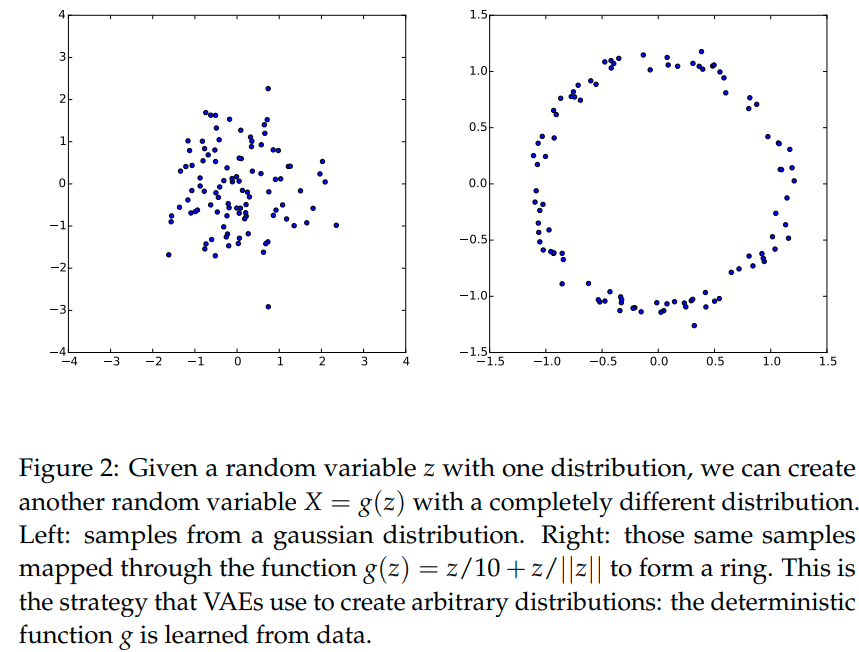
\includegraphics[height=0.3\textheight,width=0.9\textwidth,keepaspectratio]{inverseTransformSampling}   \end{figure}

  \item Conceptually, it easy to approximate $P(X)$  - we sample a large value of $z$ values $\left\{ \bm{z}_1, \ldots, \bm{z}_n \right\}$, and compute $P(X) \approx \frac{1}{n} \sum_{i} P(X| \bm{z}_i)$. 
  However, for high dimensional spaces, the number of samples of $\bm{z}$ might need to be very large before we have an accurate estimate of $P(X)$. 
  They include a reason why this is so:
\begin{figure}[H] \centering 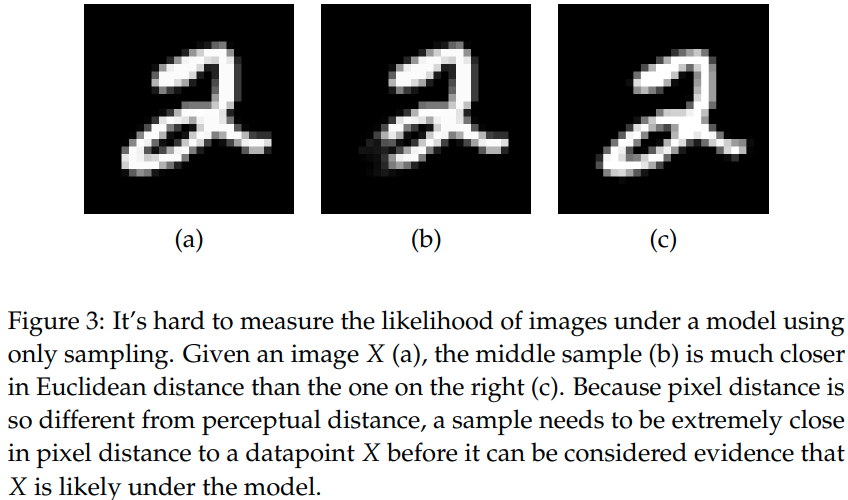
\includegraphics[height=0.3\textheight,width=0.9\textwidth,keepaspectratio]{samplingOnlyLikelihood}  \label{fig:samplingOnlyLikelihood} \end{figure}
  So instead, we use the correct assumption, that for most $\bm{z}$, $P(X|\bm{z})$ will be nearly zero, and hence contribute almost nothing to our estimate of $P(X)$. 
  Therefore, we attempt to sample values of $\bm{z}$ that are likely to have produced $X$, and compute $P(X)$ just from those.  
  This means we need a new function $Q(\bm{z}|X)$, the "recognition" model, which can take a value of $X$ and give a distribution over $\bm{z}$ values that are likely to produce $X$. 
  By assuming that this space of $\bm{z}$ values that are likely under $Q$ will be much smaller than the space of all $\bm{z}$  that are likely under the prior $P(\bm{z})$. 
  This lets us compute $E_{\bm{z} \sim Q} P(X|\bm{z})$ relatively easy. 

\end{enumerate}

We now formulate our new objective. Having moved to computing $E_{z \sim  Q}P(X | \bm{z})$, we need to relate $P(X)$ to $E_{\bm{z} \sim  Q} P(X | \bm{z})$. We use some math tricks:
\[
  \mathrm{KL} \Big[Q(\bm{z}|X) \,||\, P(\bm{z} |X) \Big] = E_{\bm{z} \sim Q} \Big[ \log Q( \bm{z}|X) - \log P(\bm{z} | X) \Big]
\]
Using Bayes rule, we get:
\[
  \mathrm{KL} \Big[ Q(\bm{z} | X) \,||\, P( \bm{z} |X)  \Big] = E_{\bm{z} \sim  Q}  \Big[ \log Q(\bm{z} | X) - \log P(X| \bm{z}) - \log P(\bm{z}) \Big] + \log P(X)
\]
We negate and move sides, and get:
\begin{equation} \label{eq:DoreschEq5}
  \log P(X) - \mathrm{KL} \Big[ Q(\bm{z} | X) \,||\, P(\bm{z} | X)  \Big] = E_{\bm{z} \sim  Q} \Big[ \log P(X| \bm{z}) \Big] - \mathrm{KL} \Big[ Q(\bm{z} | X) \,||\, P(\bm{z}) \Big]
\end{equation}

The LHS is the quantity we wish to optimize, plus an error term for how well $Q$ produces $\bm{z}$ the can reproduce a given $X$; This is small for the high-capacity $Q$. The RHS is something we can optimize via SGD. Recall that we assume that:
\[
  Q(\bm{z}|X) = \mathcal{N}\big(\bm{z} | \mu(X ; \phi), \Sigma(X ; \phi) \big)
\]
Since we also assume Gaussian prior $P(\bm{z})$, we get the value of $\mathrm{KL} \Big[ Q( \bm{z} | X) \,||\, P(\bm{z}) \Big]$. 
As For the first term, we take one sample of $\bm{z}$, and treat $\log P(X|z)$ (which we compute via $f(\bm{z} ; \theta)$ as the approximation of $E_{\bm{z} \sim  Q} \big[ \log P(X | \bm{z}) \big]$. 
Recall we are already doing stochastic gradient descent over different values of $X$ from a dataset $D$. The full equation we want to optimize is:
\begin{equation} \label{eq:DoreschEq8}
\begin{aligned}
  E_{X \sim  D} \Big[   \log P(X) - \mathrm{KL} \Big[ Q(\bm{z} | X) &\,||\, P(\bm{z} | X)  \Big] \Big] =\\
  & E_{X \sim  D} \Big[  E_{\bm{z} \sim  Q} \big[ \log P(X| \bm{z}) \big] - \mathrm{KL} \big[ Q(\bm{z} | X) \,||\, P(\bm{z}) \big] \Big] 
\end{aligned}
\end{equation}
Hence we can compute:
\[
  P(X | \bm{z}) - \mathrm{KL} \Big[ Q(\bm{z} | X) \,||\, P(\bm{z}) \Big]
\]
And we can take its gradient. By averaging the gradient of this function over aribtrarily many samples of $X$ and $\bm{z}$, the result converges to the gradient of~\cref{eq:DoreschEq8}. 


However there is still one problem.In~\cref{eq:DoreschEq8}, $E_{\bm{z} \sim  Q} \big[ \log P(X | \bm{z}) \big]$ depends both on the parameters of $P$ ($\theta$) and $Q$ ($\phi$). Doing back propagation on the (left) network below is impossible, since sampling is a non-continuous operation, and has no gradient. 
\begin{figure}[H] \centering 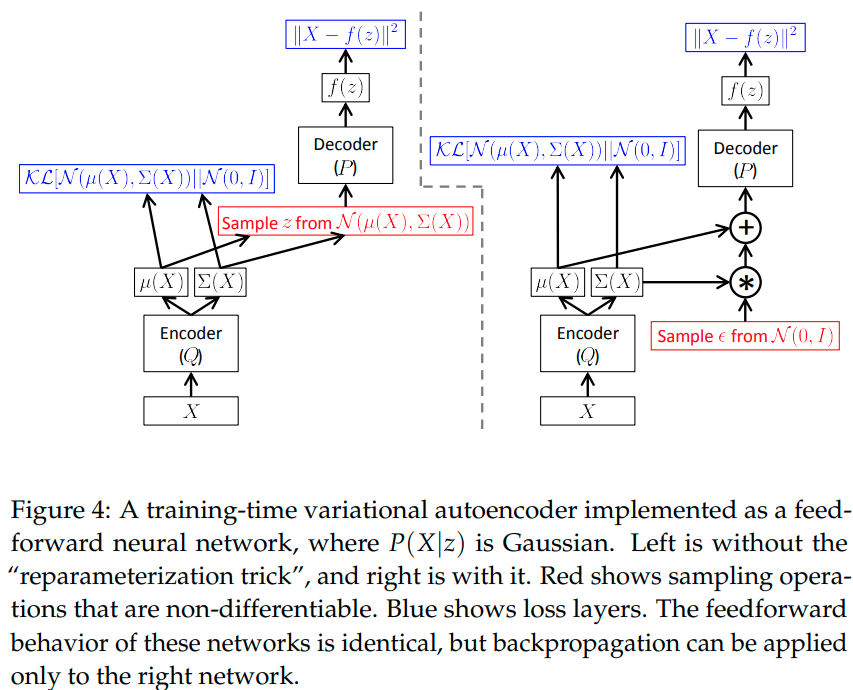
\includegraphics[height=0.3\textheight,width=0.9\textwidth,keepaspectratio]{DoreschReparamTrick} \label{fig:DoreschReparamTrick} \end{figure}

  The solution is called the reparametrization trick. We move the sampling to an input layer, $\epsilon \sim  \mathcal{N}(0, I)$, and then compute $z = \mu(X) + \Sigma^{1/2} (X) * \epsilon$, where $\mu(X), \Sigma(X)$ were computed by $Q$. 

Thus, the equation we actually take the gradient of is:
\[
  E_{X \sim  D} \Big[  E_{\epsilon \sim  \mathcal{N}(0,I)} \big[ \log P(X| \bm{z} = \mu(X) + \Sigma^{1/2} (X) * \epsilon) \big] - \mathrm{KL} \big[ Q(\bm{z} | X) \,||\, P(\bm{z}) \big] \Big] 
\]
And since this sampling is independent of $\theta$ and $\phi$, we don't need to do backpropagation over the sampling. 

\subsection{Test Time}
\begin{figure}[H] \centering 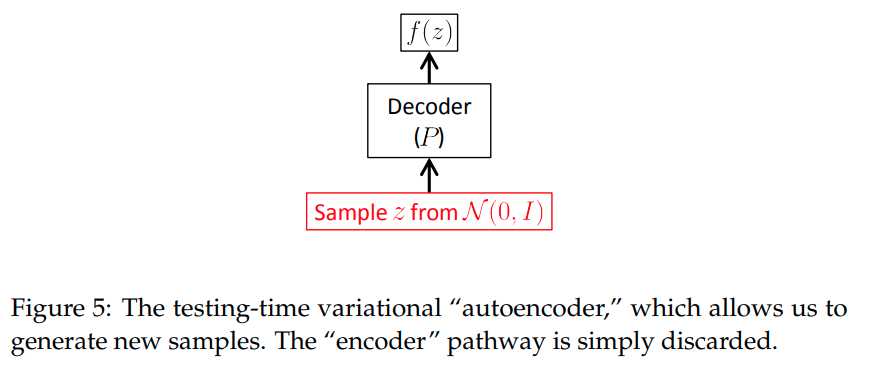
\includegraphics[height=0.3\textheight,width=0.9\textwidth,keepaspectratio]{DoreschTestTime}  \label{fig:DoreschTestTime} \end{figure}



\newpage
\section{Diagnosing and Enhancing VAE Models}
\ul{Bin Dai, David Wipf} Microsoft / Amazon / Tsinghua / 2019

We wish to learn a probabilistic generative model of observale variables $\bm{x} \in \mathcal{X}$, where $\mathbb{X}$ is an $r$-dimensional manifold embedded in $\mathbb{R}^{d}$. Moreover, we assume that $\mathcal{X}$  is a simple Riemannian manifold, which means there exists a diffeomorphism $\phi : \mathcal{X} \to \mathbb{R}^{r}$ . Denote the ground-truth probability measure on $\mathcal{X}$ as $\mu_{gt}$ such that the probability mass of an infinitesimal $\d{\bm{x}}$ on the manifold is $\mu_{gt}(\d{\bm{x}})$, and $\int_{\mathcal{X}} \mu_{gt} (\d{\bm{x}})  = 1$.

The VAE attempts to approximate this ground truth measure, using a parameterized density $p_{\theta}(\bm{x})$ defined across all of $\mathbb{R}^{d}$.
The density is further assumed to admit the latent decomposition $p_{\theta}(\bm{x}) = \int p_{\theta}(\bm{z} | \bm{x}) p(\bm{z}) \d{\bm{z}}$, where $z \in \mathbb{R}^{k}$ with $k \approx r$, and prior $p(\bm{z}) = \mathcal{N}(\bm{z} | \bm{0}, \bm{I})$. 

Ideally, we might like to minimize the negative log likelihood $- \log p_{\theta}(\bm{x})$ averaged across the ground-truth measure $\mu_{gt}$. i.e.:
\[
  \min_{\theta} \int_{\mathcal{X}} - \log p_{\theta}(\bm{x}) \mu_{gt} \left( \d{\bm{x}} \right)
\]
Unfortunately, the required marginalization over $\bm{z}$ is generally infeasible. Instead, the VAE model relies on tractable \textit{encoder} $q_{\phi}(\bm{z} | \bm{x})$ and \textit{decoder} $p_{\theta}(\bm{x} | \bm{z})$ distributions, where $\phi$ represents additional trainable parameters. 

The canonical VAE can be written as:
\[
  \mathcal{L}(\theta, \phi) := \int_{\mathcal{X}} \Big\{ - E_{q_{\phi}(\bm{z} | \bm{x})} \left[ \log p_{\theta}(\bm{x} | \bm{z}) \right] + KL[q_{\phi}(\bm{z} | \bm{x})] \Big\} \mu_{gt}(d \bm{x}) 
\] 

\section{Summary}
Assume we have $n$ data vectors (e.g. images),  $\bm{x}_1, \ldots  \bm{x}_n$, each $\bm{x}_i \in \mathbb{R}^{d}$. 
We assume the data was generated via a latent variable model: There is a latent space $\mathcal{Z} \subseteq \mathbb{R}^{k}$, and $\bm{z} \sim p_{\bm{z}}$. 
We assume there is some continuous, invertible function $\bm{f} : \mathcal{Z} \to \mathcal{X}$, that generates the data, i.e.  $\bm{f}(\bm{z}) = \bm{x}$. 
This induces a distribution $p ^{\ast}(\bm{x})$ over the data space $\mathcal{X}$, which we wish to learn / estimate from the observed data $\bm{x}_1, \ldots, \bm{x}_n$. 
We assume $p ^{\ast}(\bm{x})$ belongs to some parametric family $\Theta$, and we wish to learn $\theta$ of $p_{\theta}(\bm{x})$. 

Unfortunately, common methods like MLE can estimate $\theta$ only when $\Theta$ is a very simple family (like Gaussian), which is an unrealistic assumption for images. 



\end{document}

